\section{Metodologia}
\label{sec:metodologia}

Spiegare notazione grafo, parametri, usiamo 1 simbolo per indicare gli score. Quando scriviamo una sezione qui sotto 2.x, se ci serve della notazione poi andiamo a metterla qui. 
Fare dei paragrafi per BM25, PageRank, Hits, LSA, ES.

%In questo paragrafo, si illustreranno i metodi sviluppati e sperimentati con le
%attivit\`a di laboratorio. Le notazioni e tutti gli aspetti non banali dovranno
%essere spiegati. Naturalmente, la notazione di un paragrafo non dovr\`a essere
%reintrodotta nei paragrafi successivi, di conseguenza, la notazione non dovr\`a
%essere ambigua.

\subsection{Approccio}
\label{sec:approccio}

Il nostro scopo e' ottenere un valore di map il piu' elevato possibile. Per calcolarla e verificarne il cambiamento durante le varie versione del codice utilizziamo \texttt{treceval}, esso e' il tool standard usato dalla \"TREC community\" per valutare un'esecuzione ad hoc, dandole il file contenete i risultati e un set standard di risultati giudicati.  

Abbiamo optato approccio probabilistico per la risoluzione dei laboratori, poiche' fornisce una formalizzazione piu' pulita di cosa volgiamo che faccia un sistema IR: dare documenti rilevanti agli utenti. 
Inoltre per via delle nostre conoscenze abbiamo voluto utilizzare il linguaggio Python per dare corpo ai progetti. Inoltre vi sono diverse librerie che implementano molti metodi utili per tale corso e per garantire buone performance al codice: \texttt{numpy} usata per la gestione delle matrici, \texttt{matplotlib} utilizza per effettuare i plot (grafici) dei risultati ottenuti, \texttt{networkx} utilizzata per la creazione e gestione dei grafi.
Oltre a \texttt{Python} abbiamo utilizzato altri software per il lavoro. E' stato usato \texttt{Git}, e' un sistema di versionamento distribuito, per lo scambio del codice e l'aggiornamente delle diverse versioni di quest'ultimo. Infine \texttt{latex} per la scrittura dei pdf di report.
Per ogni esercitazioni è stato utilizzato un approccio di gruppo. Dopo la prima sessione di laboratorio di ogni esercitazione ci siamo ritrovati per la scrittura del codice, la discussione sui risultati e la stesione del report.

\subsection{Indicizzazione} \label{sec:metodi-di-indic}

\textbf{Descrizione}: comprensione dei meccanismi di indicizzazione e costruzione di un algoritmo di indicizzazione.
\textbf{Implementazione}: come base di partenza abbiamo tre diversi file contenenti: \begin{enumerate}\item frequenza delle parole stemmate
 \item la stoplist 
 \item le keywords per ogni documento
  \end{enumerate}
Vogliamo estrarre i pesi tf-idf dei termini dataci la collezione e produrre in output un file che li contenga, quest'ultimo sara' formattato nel seguente modo: 
word1  doc_id  weight
word2  doc_id  weight
...
Poiche' le stop words sono gia' state rimosse dalle keywords, ci permettiamo di ignorare la stoplist, inoltre le keywords sono gia' state stemmate quindi possiamo ignorare anche il file che contiene le stemmature.
L'algoritmo scritto costruisce una dizionario, costituito dalle parole uniche, dopo di che' forma una matrice con numero di colonne pari al numero di documenti e come righe il numero di parole, contenente l'occorrenza, usando il file delle frequenze. Avendo la matrice utilizza la \textit{TfidfTransformer} del modulo scikit-learn per ottenere una matrice dei pesi tf-idf e salvarla nel file di output.

\subsection{Reperimento}
\label{sec:metodi-di-reper}

\textbf{Descrizione}: comprensione dei meccanismi di reperimento e costruzione di un primo algoritmo di reperimento
\textbf{Implementazione}: abbiamo studiato ed utilizzato l'algoritmo di ranking Okapi BM25. Per poterlo implementare necessitiamo della matrice delle frequenze di grandezza \textit{n documenti} X \textit{n parole} e di un array contenente le lunghezze dei vari documenti.
La nostra funzione di reperimento è cosi' composta: per ogni query $Q$ scorrera' la lista dei documenti (cioe' le righe della matrice) e per ognuno di essi scorre i termini della query calcolandone gli score, infine ordina in modo decrescente i documenti aventi punteggi maggiori di zero.
\begin{algorithmic}
\State $Q \gets query$
\ForAll{$doc \in C$} 
    \State $score\gets 0$
    \ForAll{$qw \in Q$}
        \State $score \gets score + f_{bm25}(doc, qw)$
    \EndFor
\EndFor\\
\Return top $k$ scoring documents
\end{algorithmic}
Tale algoritmo ha complessita' $O(n \cdot m)$, dove $n$ e' il numero di documenti nella collezione ed $m$ e' il numero di descrittori nell'interrogazione (query) $Q$.

\subsection{Relevance Feedback}
\label{sec:relevance-feedback}

\textbf{Descrizione}: comprensione del \textit{Relevance Feedback} (RF) e scrittura di una funzione di reperimento equipaggiata con \textit{RF esplicito} e una seconda con \textit{RF pseudo}.

\textbf{Implementazione}: durante il calcolo di BM25 terremo conto dei giudizi di rilevanza, per quanto riguarda il caso di feedback esplicito verra' utilizzato il file \textit{qrels-treceval.txt}.
BM25:
\[ \sum\limits_{i \in Q}\log\Bigl(\frac{(r_i+0.5)/(R-r_i+0.5)}{(n_i-r_i+0.5)/(N-n_i-R+r_i+0.5)}\Bigl)\cdot\frac{(k_1+1)f_i}{k+f_i}\cdot\frac{(k_2+1)qf_i}{k_2+qf_i}. \]
La formula di BM25 tiene gia' in considerazione i giudizi di rilevanza, infatti $R$ rappresenta il numero di documenti rilevanti per la query presa in considerazione, mentre il valore di $r_i$ rappresenta il numero di documenti rilevanti che contengono il termine $i$.
Il procedimento si suddivide in due passi sia per il calcolo del \tetxtit{Relevance Feedback Esplicito} sia per \textit{Pseudo Relevance Feedback}.
Il primo passo e' comune e consiste nel calcolo del ranking senza informazioni di rilevanza, il secondo passo differisce:
\begin{enumerate}
\item \textbf{Relevance Feedback Esplicito}: tra i primi $N$ documenti verranno estratti quelli ritenuti rilevanti utilizzando il file \texttt{qrels-treceval.txt}, da tali documenti verranno estratti i valori di $R$ ed $r_i$ che saranno usati per la seconda esecuzione dell'algoritmo.
\item \textbf{Pseudo Relevance Feedback}: verranno considerati rilevanti i primi $N$ documenti, con tali documenti verranno trovati i valori di $R$ ed $r_i$ utilizzati per la seconda esecuzione dell'algoritmo.
\end{enumerate}
Per poter effettuare il calcolo dei valori di $R$ ed $r_i$ l'algoritmo utilizzera' le frequenze di occorrenza delle parole per ogni documento (contenute in una matrice di grandezza $n_docs$ X $n_words$). Durante il reperimento per ogni documento e per ogni termine $i$ l'algoritmo calcola il numero di documenti considerati rilevanti che lo contengono e salvera' tale valore in una mappa $map$ (mappa $i$->$r_i$), con questa mappa l'algoritmo calcola il ranking rispetto ai valori di $R$ ed $r_i$.


\subsection{PageRank}
\label{sec:pagerank}

\textbf{Descrizione}: comprensione di PageRank, implementazione di PageRank e scrittura di una funzione di reperimento che lo integri.

\textbf{Implementazione}: la funzione di reperimento combinera' gli score di BM25 ($rk$) con il valore del pagerank ($pr$) attraverso la seguente formula:

\[ score =  \alpha \cdot rk + (1-\alpha) \cdot pr,\]

dove $\alpha$ e' un parametro che varia tra 0 ed 1 e, quindi, sposta il peso uniformemente da pagerank a BM25.
Ma poter effettuare questo confronto in modo coerente, entrambe le distribuzioni devono essere ridimensionate, si effettua quindi una normalizzazione in modo da avere valori compresi tra 0 e 1. Per far cio' abbiamo usato la formula:

\[ z_i = \frac{x_i - min(x)}{max(x) - min(x)}, \]

Per effettuare il calcolo del pagerank abbiamo utilizzato la libreria \texttt{networkx}, essa attraverso il metodo \texttt{read_edgelist} permette la costruzione del grafo delle citazione a partire dalla lista 	di archi. Inoltre dispone del metodo \texttt{pagerank} per la computazione del pagerank utilizzando \textit{power iteration} sulla matrice di transizione, tale computazione e' fatta a tempo di indexing e i valori verranno utilizzati a tempo di retrieval.
\subsection{Latent Semantic Analysis}
\label{sec:lsa}

\textbf{Descrizione}: comprensione di Latent Semantic Analysis (LSA), implementazione di LSA e costruzione di una funzione di reperimento che implementi LSA.

\textbf{Implementazione}: come funzione di ranking sara' usata la BM25 con relevance feedback esplicito (laboratorio 5) e verra' applicata LSA. 
L'algoritmo calcolera' quindi la BM25 con relevance feedback esplicito e prendera' in considerazione soltanto i primi $N$ documenti reperiti. Utilizzera' il metodo \texttt{linalg.svd} (appartenente alla libreria \texttt{numpy}) per il calcolo della fattorizzazione della matrice termini-documenti $X$: 
\[ X = U \Sigma V^{T}. \]\\
Da questa matrice derivera' la matrice ridotta tenendo in considerazione soltanto $m$ dimensioni. Di seguito effettuera' la proiezione di $\vec{q}$ sullo spazio a dimensione ridotto secondo la formula: 
\[ \vec{q}_m = \Sigma^{-1}_m U^{T}_m \vec{q}. \]

Infine computera' la \textit{cosine similarity} tra le rappresentazione degli $N$ documenti nello spazio ridotto (cioe' le colonne $V_m^{T}$) e la query ridotta $\vec{q}$, riordinera' i risultati di questi $N$ documenti in ordini decrescente e ad essi verranno accodati i restanti documenti calcolati ad inizio algoritmo tramite BM25 con relevance feedback esplicito.


\subsection{Hyper-linked Induced Topic Search}
\label{sec:hits}

\textbf{Descrizione}: comprensione di Hyperlinked Induced Topic Search (HITS), implementazione e costruzione di una funzione di reperimento che implementi HITS.

\textbf{Implementazione}: l'algoritmo da noi scritto effettuera' il ranking tramite la funzione BM25 (laboratorio 3), attraverso i primi $N$ documenti costruisce il grafo delle citazioni $R_q$. Quest'ultimo verra' espanso per ottenere un grafo allargato $B_q$ sul quale sara' calcolato \textit{HITS}.
Infine combinera', per i primi $N$ documenti, gli score di BM25 (\texttt{sc}) con i punteggi di authority (\texttt{auth}) e hubbiness (\texttt{hub}) attraverso la formula:
\[ hits_{score} =  \alpha \cdot sc + \beta \cdot auth + \gamma \cdot hub,\]

Il valore del parametro $\alpha$ varia in [0, 1],  mentre quello di $\beta$ e $\gamma$ puo' variare tra [-1, 1], in quanto si vogliono cogliere possibili influenze negative, mentre i valori di $sc, auth, hub$ vengono normalizzati in [0, 1] prima del calcolo. 
Infine l'algoritmo riordina in modo decrescente per $hits_score$.

\subsection{Evolution Strategy}
\label{sec:es}

Per ottimizzare gli algoritmi di reperimento abbiamo scelto di utilizzare un Evolution Strategy~\cite{back1996evolutionary} (ES) che e' una tecnica di ottimizzazione basata sui principi che regolano l'evoluzione. Tecniche di questo tipo sono piu' robuste rispetto ai metodi di ricerca lineare per quanto riguardo i massimi locali. Il loro svantaggio consiste nel maggior numero di valutazioni richieste. Nel nostro contesto una valutazione impiega circa 3-15 secondi a seconda della complessita' del metodo di reperimento. Cio' permette di eseguire l'algoritmo di ottimizzazione in un tempo accettabile.

I parametri che abbiamo scelto di ottimizzare cambiano in base alla funzione di reperimento (e quindi del laboratorio). Per il laboratorio 3, 4, 6 abbiamo scelto di ottimizzare $k_1, b$. Ignoriamo $k_2$ in quando abbiamo visto che non ci sono termini ripetuti nelle query e quindi tale termine non influisce sul punteggio. Per il laboratorio 5 ottimizziamo $k_1, b, \alpha$. Per il laboratorio 7 ottimizziamo $k_1, b, \alpha, \beta, \gamma$. Per lo pseudo relevance feedback del laboratorio 4 il numero di documenti considerati rilevanti $R = 50$, mentre per l'\textsc{lsa} del laboratorio 6 il numero di documenti da riordinare $N = 30$, e il numero di dimensioni per la riduzione $m=2$ (tali parametri sono interi e non si prestano ad un ottimizzazione tramite ES). La funzione da massimizzare e' la Mean Average Precision.

Figura \ref{fig:es_all} riporta l'andamento della MAP durante l'ottimizzazione della funzione di reperimento dei laboratori. 
\begin{figure*}
        \centering
        \begin{subfigure}[htpb]{0.475\textwidth}
            \centering
            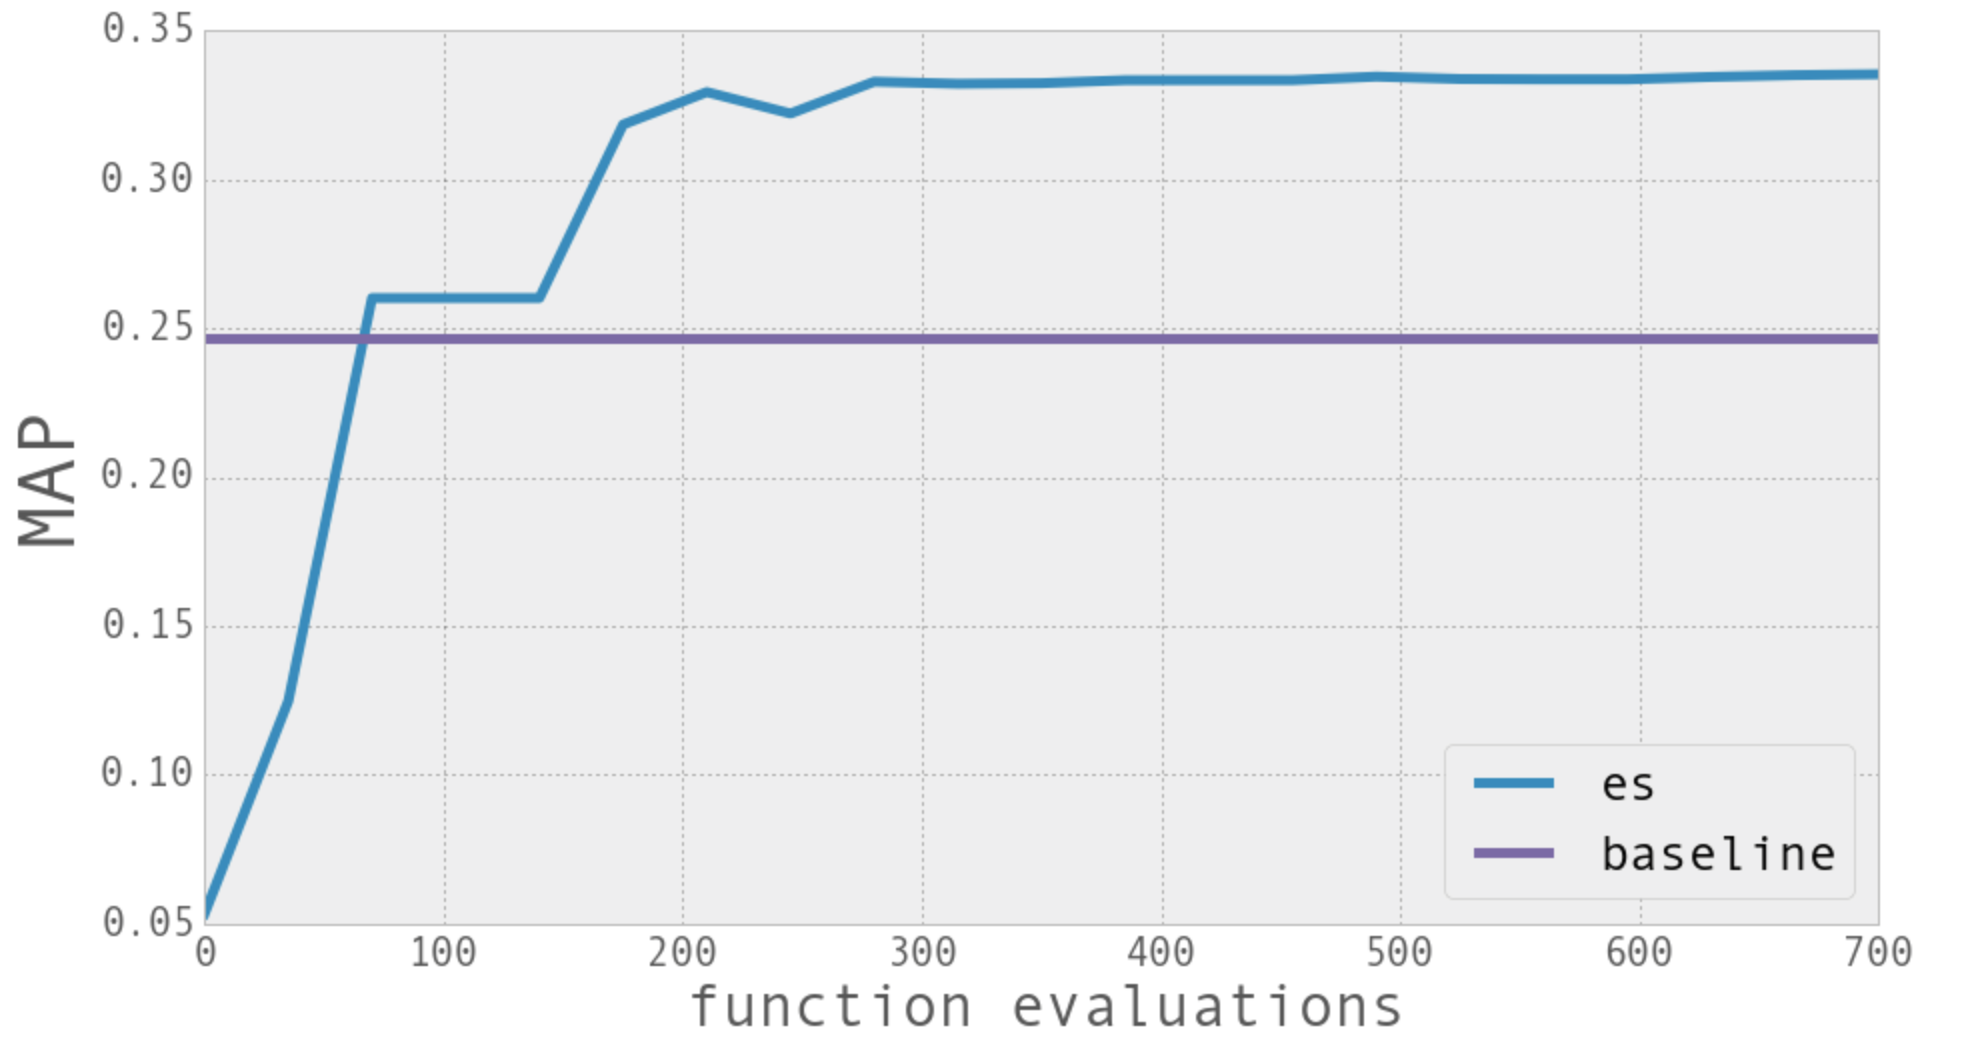
\includegraphics[width=\textwidth]{figures/es_lab3.png}
            \caption[Network2]%
            {{\small Laboratorio 3 (\textsc{baseline})}}    
            \label{fig:es_lab3}
        \end{subfigure}
        \hfill
        \begin{subfigure}[htpb]{0.475\textwidth}  
            \centering 
            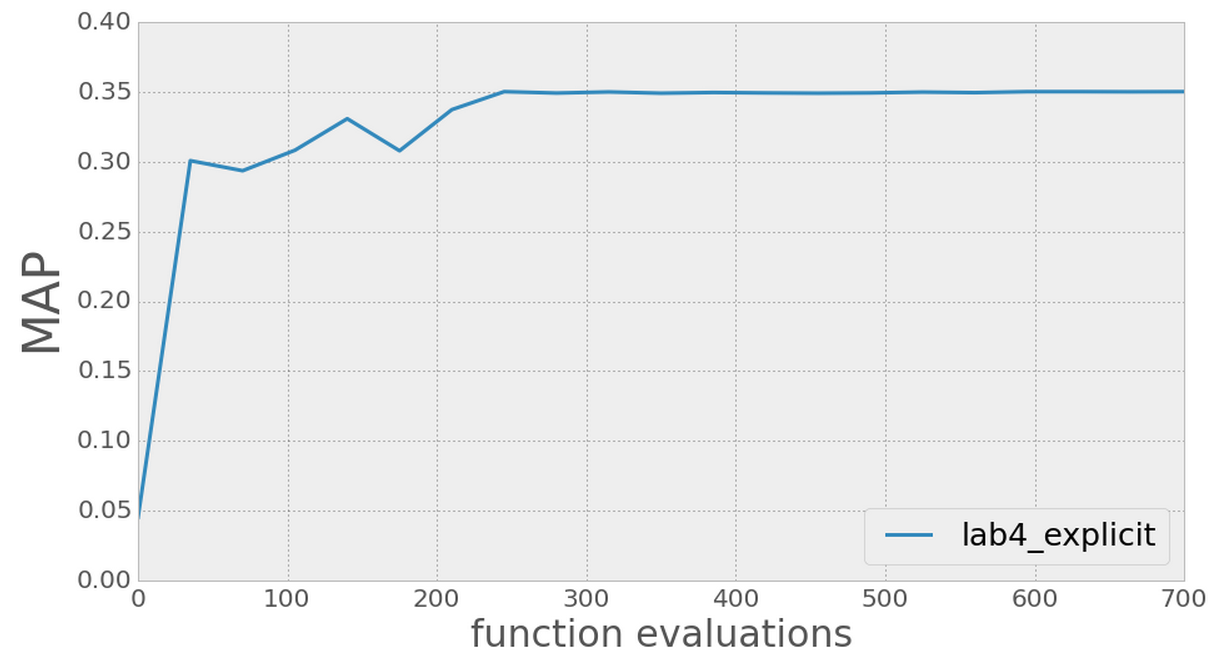
\includegraphics[width=\textwidth]{figures/es_lab4_e.png}
            \caption[]%
            {{\small Laboratorio 4 (\textsc{RF} esplicito)}}    
            \label{fig:es_lab4_esp}
        \end{subfigure}
        \vskip\baselineskip
        \begin{subfigure}[htpb]{0.475\textwidth}   
            \centering 
            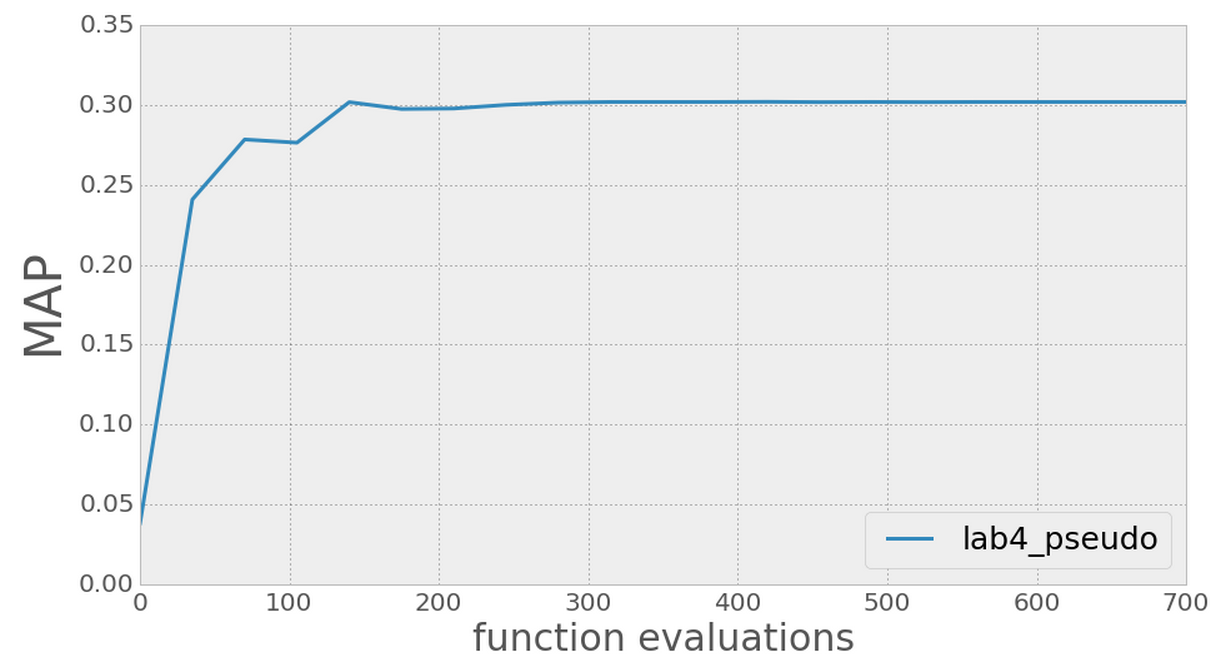
\includegraphics[width=\textwidth]{figures/es_lab4_p.png}
            \caption[]%
            {{\small Laboratorio 4 (\textsc{RF} pseudo)}}    
            \label{fig:es_lab4_pse}
        \end{subfigure}
        \quad
        \begin{subfigure}[htpb]{0.475\textwidth}   
            \centering 
            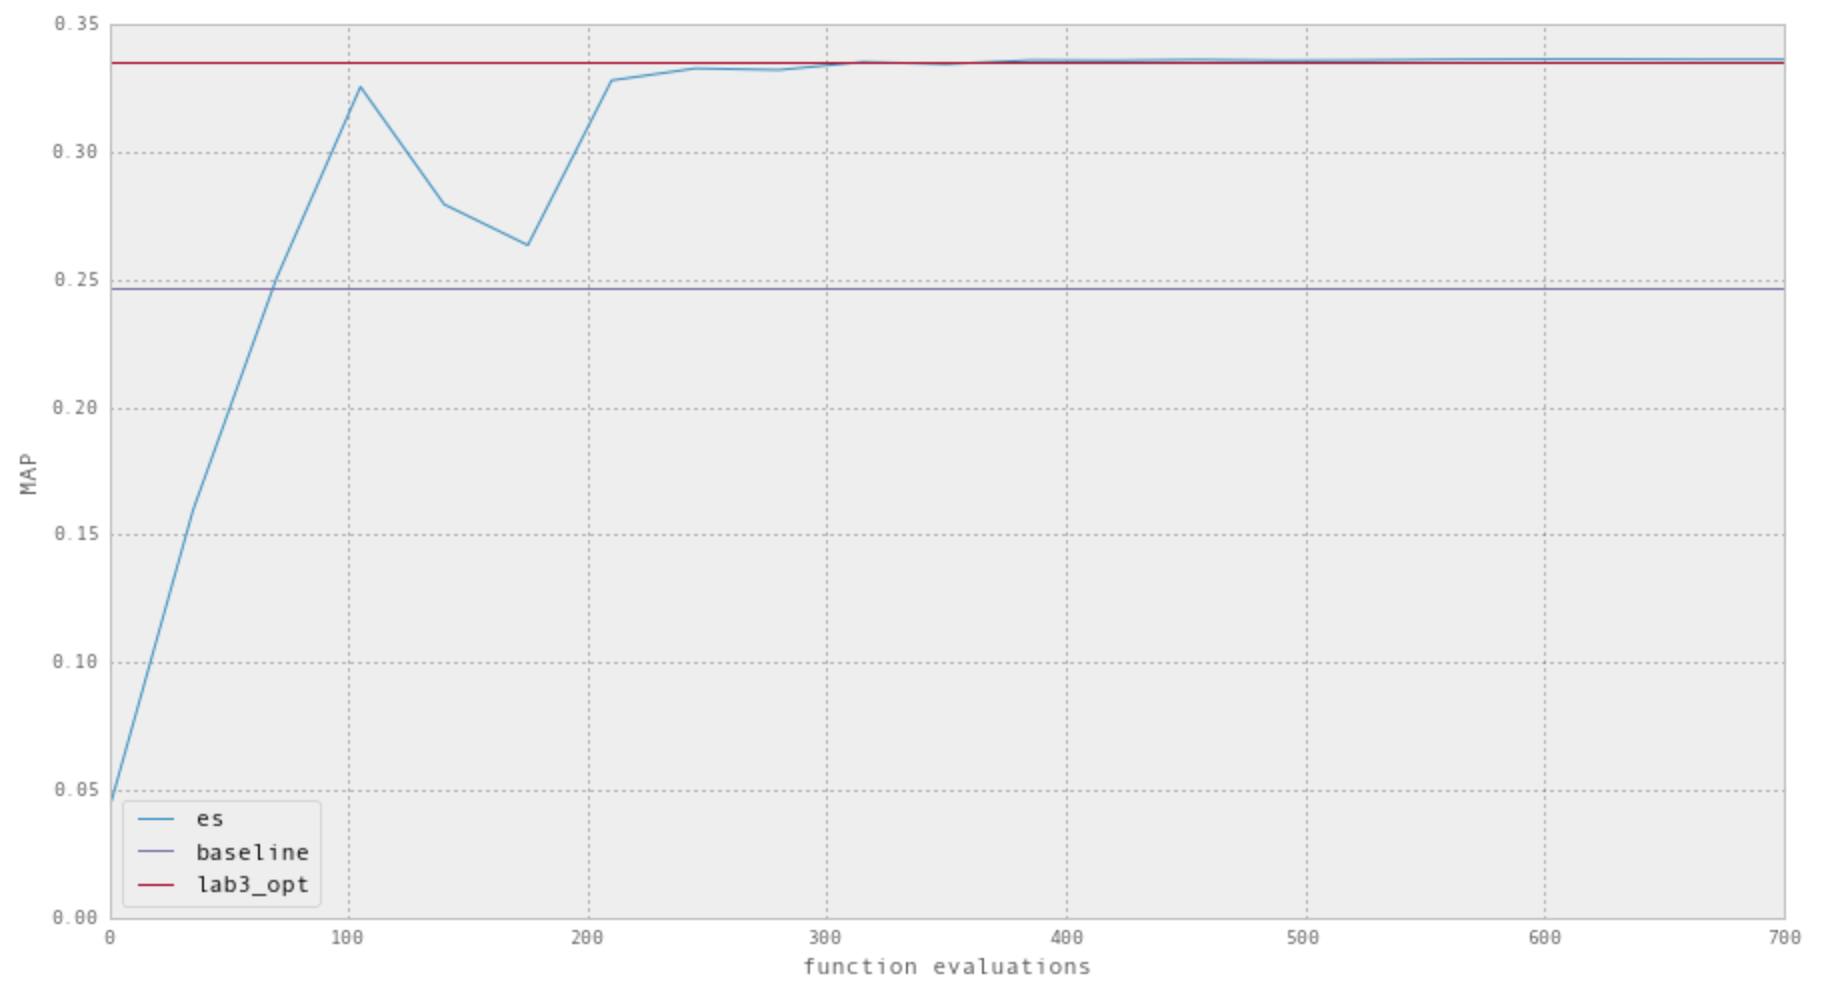
\includegraphics[width=\textwidth]{figures/es_lab5.png}
            \caption[]%
            {{\small Laboratorio 5 (\textsc{pagerank})}}    
            \label{fig:es_lab5_esp}
        \end{subfigure}
        \vskip\baselineskip
        \begin{subfigure}[htpb]{0.475\textwidth}  
            \centering 
            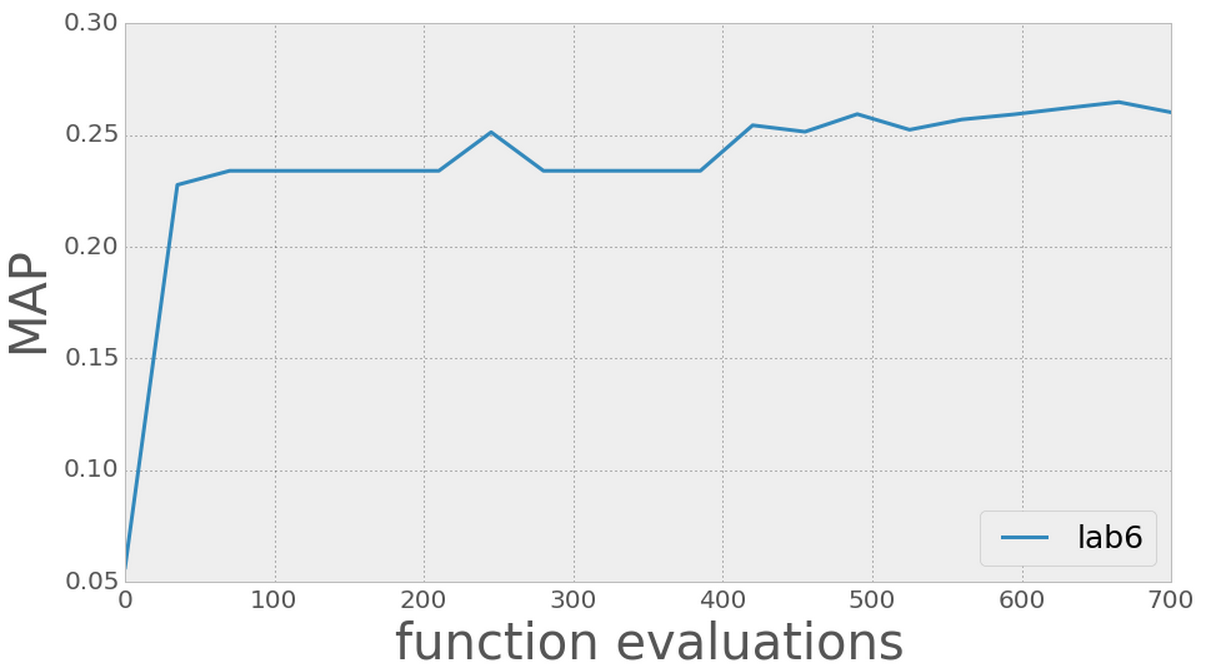
\includegraphics[width=\textwidth]{figures/es_lab6.png}
            \caption[]%
            {{\small Laboratorio 6 (\textsc{lsa})}}    
            \label{fig:es_lab6}
        \end{subfigure}
        \quad
        \begin{subfigure}[htpb]{0.475\textwidth}   
            \centering 
            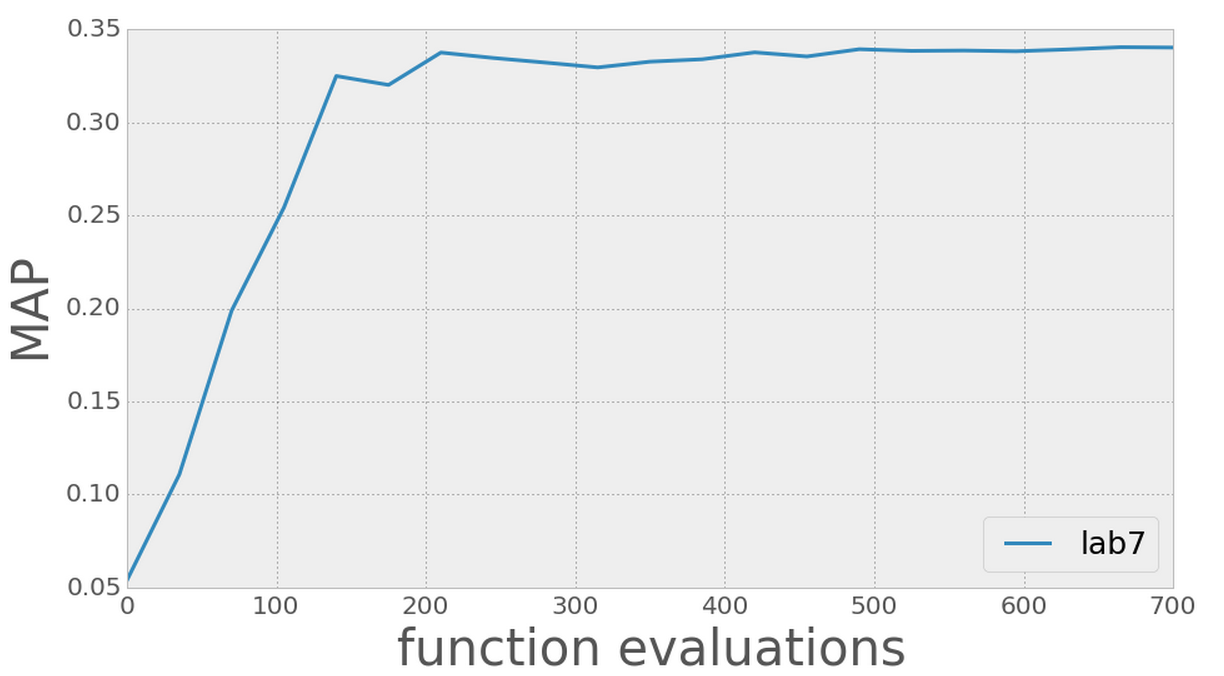
\includegraphics[width=\textwidth]{figures/es_lab7.png}
            \caption[]%
            {{\small Laboratorio 7 (\textsc{hits})}}    
            \label{fig:es_lab7}
        \end{subfigure}
        \caption[ The average and standard deviation of critical parameters ]
        {\small Valore MAP durante iterazioni dell'ES, per le funzioni di reperimento dei vari laboratori.} 
        \label{fig:es_all}
\end{figure*}
Tabella \ref{tab:es} riporta i risultati dell'ottimizzazione.
\begin{table}[htpb]

\begin{center}
\begin{tabular}{|c|c|c|}
\hline
metodo & parametri ottimizzati & MAP \\
 \hline
\textsc{baseline} & $k_1 = 0.0253, b = 0.0221$ & $0.3354$ \\
\textsc{rf} esplicito & $k_1 = 0.02065, b = 0.0$ & $0.3504$ \\
\textsc{rf} pseudo & $k_1 = 0.02065, b = 0.0$ & $0.3022$ \\
\textsc{pagerank} & $k_1 = 0.0237, b = 0.0, \alpha=0.7832$ & $0.3366$ \\
\textsc{lsa} & $k_1 = 0.0087, b = 0.0$ & $0.2648$ \\
\textsc{hits} & $k_1 = 0.0247, b = 0.0185, \alpha=1.0, \beta=0.1098, \gamma=0.0549$ & $0.3405$ \\
\hline
\end{tabular}
\end{center}
\caption{Risultati ottimizzazione con ES per le funzioni di reperimento dei vari laboratori.}
\label{tab:es}
\end{table}

Grazie all'ES si e' ottenuto un notevole miglioramento rispetto alla prima versione dove i parametri sono stati scelti empiricamente, e la MAP si aggirava attorno al $0.25$. Inoltre dai grafici si puo' notare come l'algoritmo di ottimizzazione sia molto robusto, dato che dopo $\sim{300}$ valutazioni e' gia' molto vicino alla configurazione ottima. I risultati dell'ottimizzazione vengono discussi in Sezione \ref{sec:risult-sper}.

\subsection{Altri metodi}
tipo lucene
\label{sec:altri-metodi}

Se sono stati sviluppati altri metodi, descriverli qui.

